\chapter{Estado del arte}

\section{Panorama general}

El estado del arte en reducci\'on de ruido en im\'agenes astron\'omicas muestra un desplazamiento claro desde m\'etodos cl\'asicos (wavelets, variacionales, priors expl\'icitos) hacia arquitecturas profundas con modelado probabil\'istico (U-Net, Transformers y difusi\'on), pero con una tensi\'on metodol\'ogica persistente: mejorar la calidad visual no garantiza preservar la validez cient\'ifica de la inferencia downstream \cite{elad2023revolution, vojtekova2020unet, shirasaki2021noise, akhaury2025joint, guo2026detection}.

En este trabajo, el foco no es presentar otro m\'etodo aislado de reducci\'on de ruido, sino consolidar una base comparativa reproducible para LSST/DC2 donde la evaluaci\'on se centre en impacto cient\'ifico medible (detecci\'on, fotometr\'ia, forma, sesgo) y no solo en fidelidad perceptual.

\section{Proceso de cribado y s\'intesis (PRISMA + RAG)}

La revisi\'on se reconstruy\'o de forma transparente sobre un corpus inicial de 304 PDFs, combinando aprendizaje activo (ASReview), re-ranqueo sem\'antico con RAG y verificaci\'on manual de metadatos en PDF. El uso de RAG se limit\'o a priorizaci\'on y trazabilidad sem\'antica de relaciones complejas (m\'etricas, tareas, sesgos), mientras que la decisi\'on final de inclusi\'on/exclusi\'on fue auditada manualmente.

\begin{mermaid}[width=0.95\linewidth, caption={Diagrama PRISMA del cribado (corpus astron\'omico de reducci\'on de ruido)}, pos=t]
flowchart TD
    A[Registros identificados\\nPDFs recuperados: n = 304]
    B[Cribado semantico\\nASReview + RAG sobre titulos/abstracts\\nRegistros cribados: n = 304]
    C[Exclusiones\\nNo astronomico / irrelevante / PDF no util\\nExcluidos: n = 254]
    D[Incluidos en sintesis cualitativa\\nTop-50 final curado\\nIncluidos: n = 50]
    A --> B
    B --> C
    B --> D
\end{mermaid}

\subsection{Criterios de inclusi\'on y exclusi\'on}

\textbf{Inclusi\'on}: trabajos con evaluaci\'on de reducci\'on de ruido/deconvoluci\'on sobre im\'agenes astron\'omicas (\'optico o dominios cercanos), con reporte de m\'etricas cuantitativas y/o impacto en tareas cient\'ificas (detecci\'on, fotometr\'ia, morfolog\'ia, weak lensing).\\
\textbf{Exclusi\'on}: estudios fuera del dominio astron\'omico y trabajos sin validaci\'on emp\'irica relevante.

\subsection{Estad\'isticas del corpus final}

\begin{table}[H]
    \centering
    \caption{Composici\'on del corpus final (n=50)}
    \begin{tabular}{lcc}
        \toprule
        Grupo & Conteo & Proporci\'on \\
        \midrule
        N\'ucleo astron\'omico (reducci\'on de ruido/deconvoluci\'on) & 31 & 62\% \\
        Reviews/surveys & 8 & 16\% \\
        M\'etodos de soporte (difusi\'on, Poisson, PnP, etc.) & 11 & 22\% \\
        \bottomrule
    \end{tabular}
\end{table}

\begin{figure}[H]
    \centering
    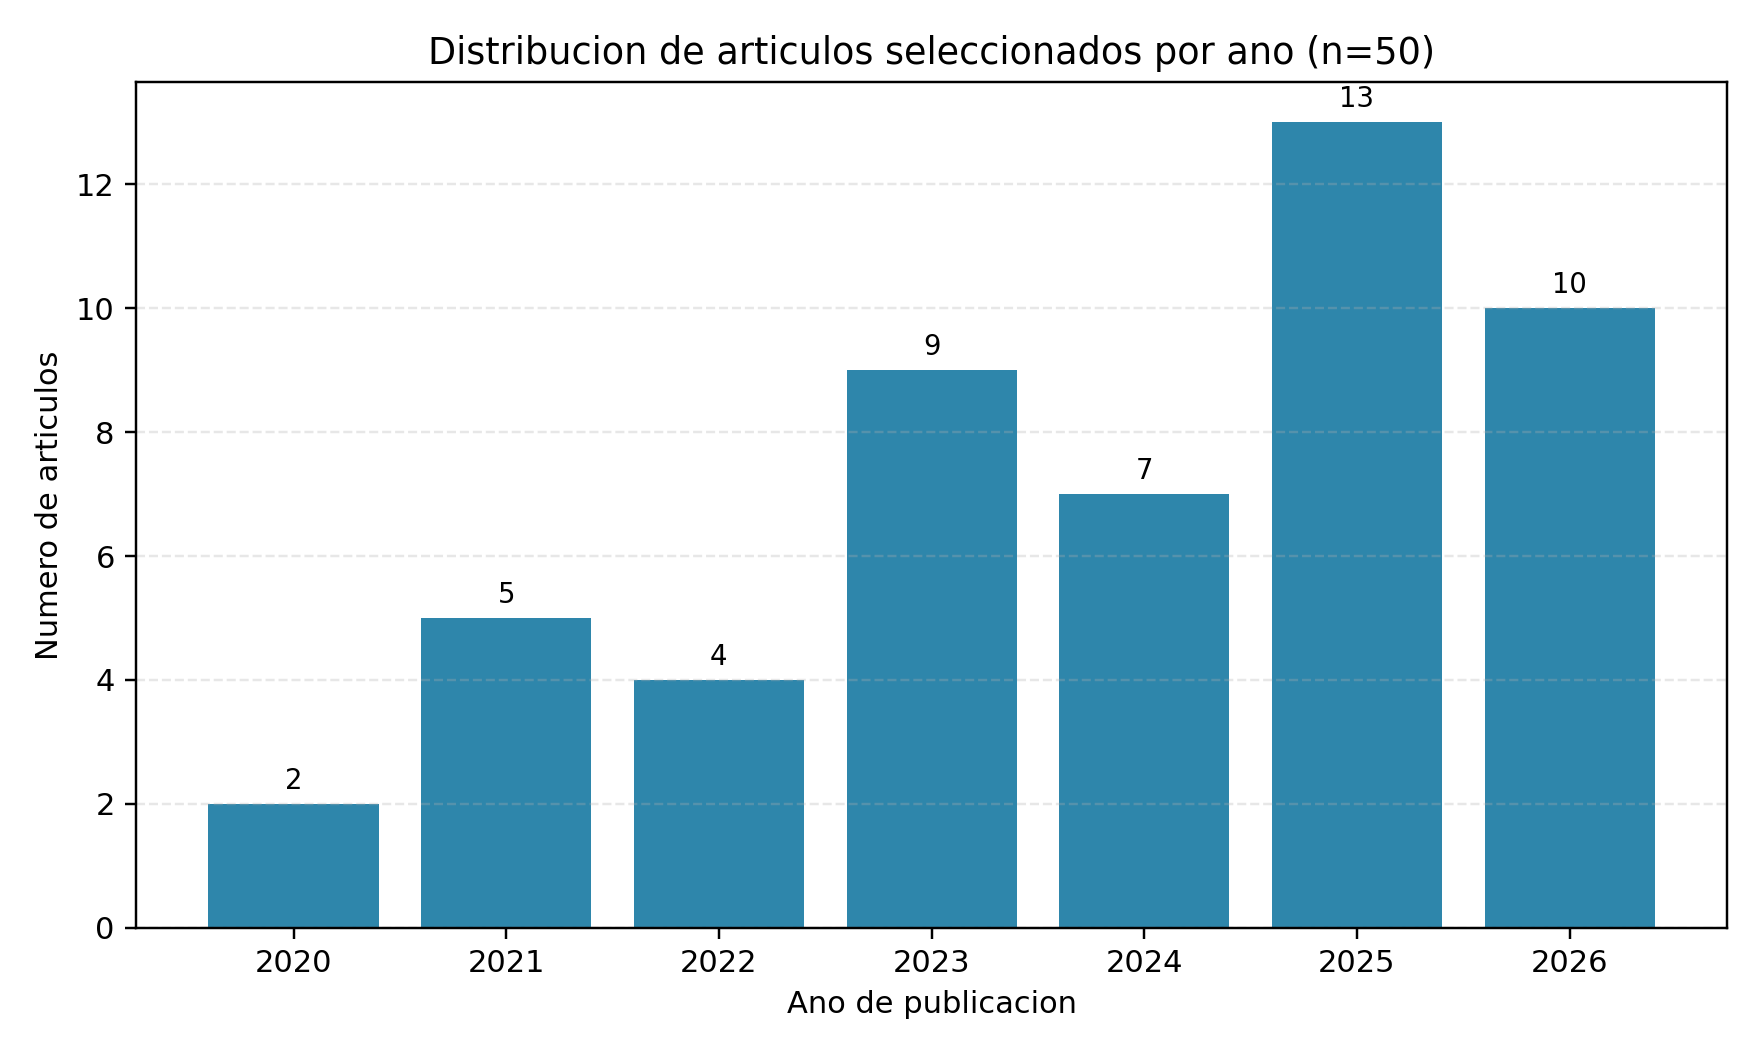
\includegraphics[width=0.9\linewidth]{assets/images/estado_arte_distribucion_anio.png}
    \caption{Distribuci\'on de art\'iculos seleccionados por a\~no (n=50).}
\end{figure}

\begin{figure}[H]
    \centering
    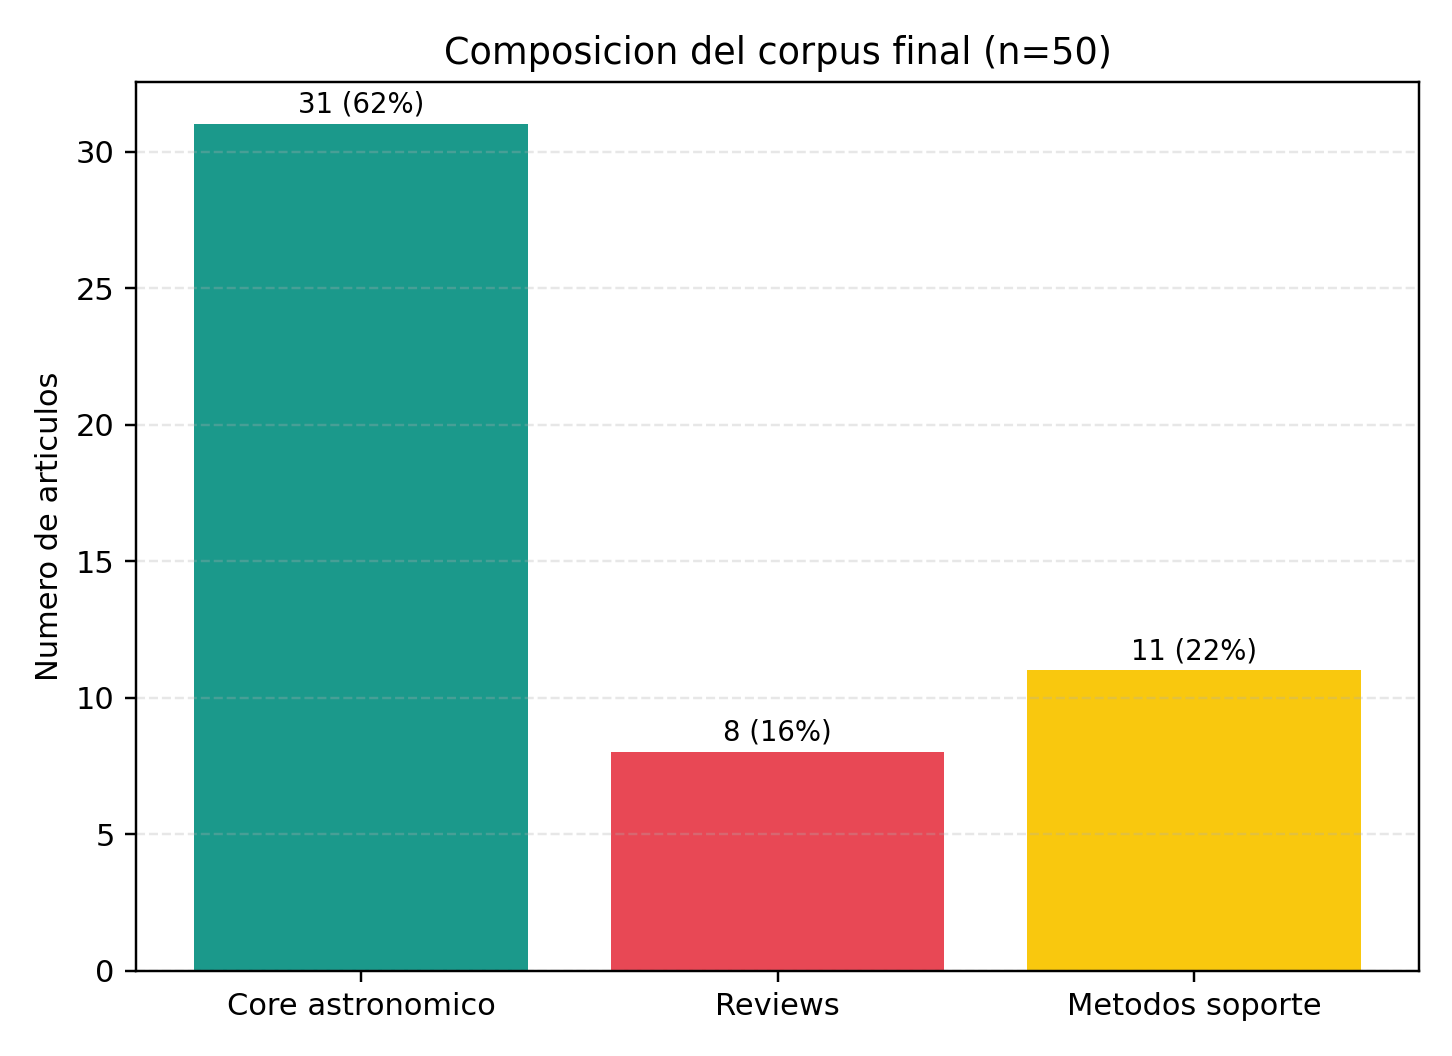
\includegraphics[width=0.8\linewidth]{assets/images/estado_arte_composicion_corpus.png}
    \caption{Composici\'on del corpus final por categor\'ia.}
\end{figure}

\begin{figure}[H]
    \centering
    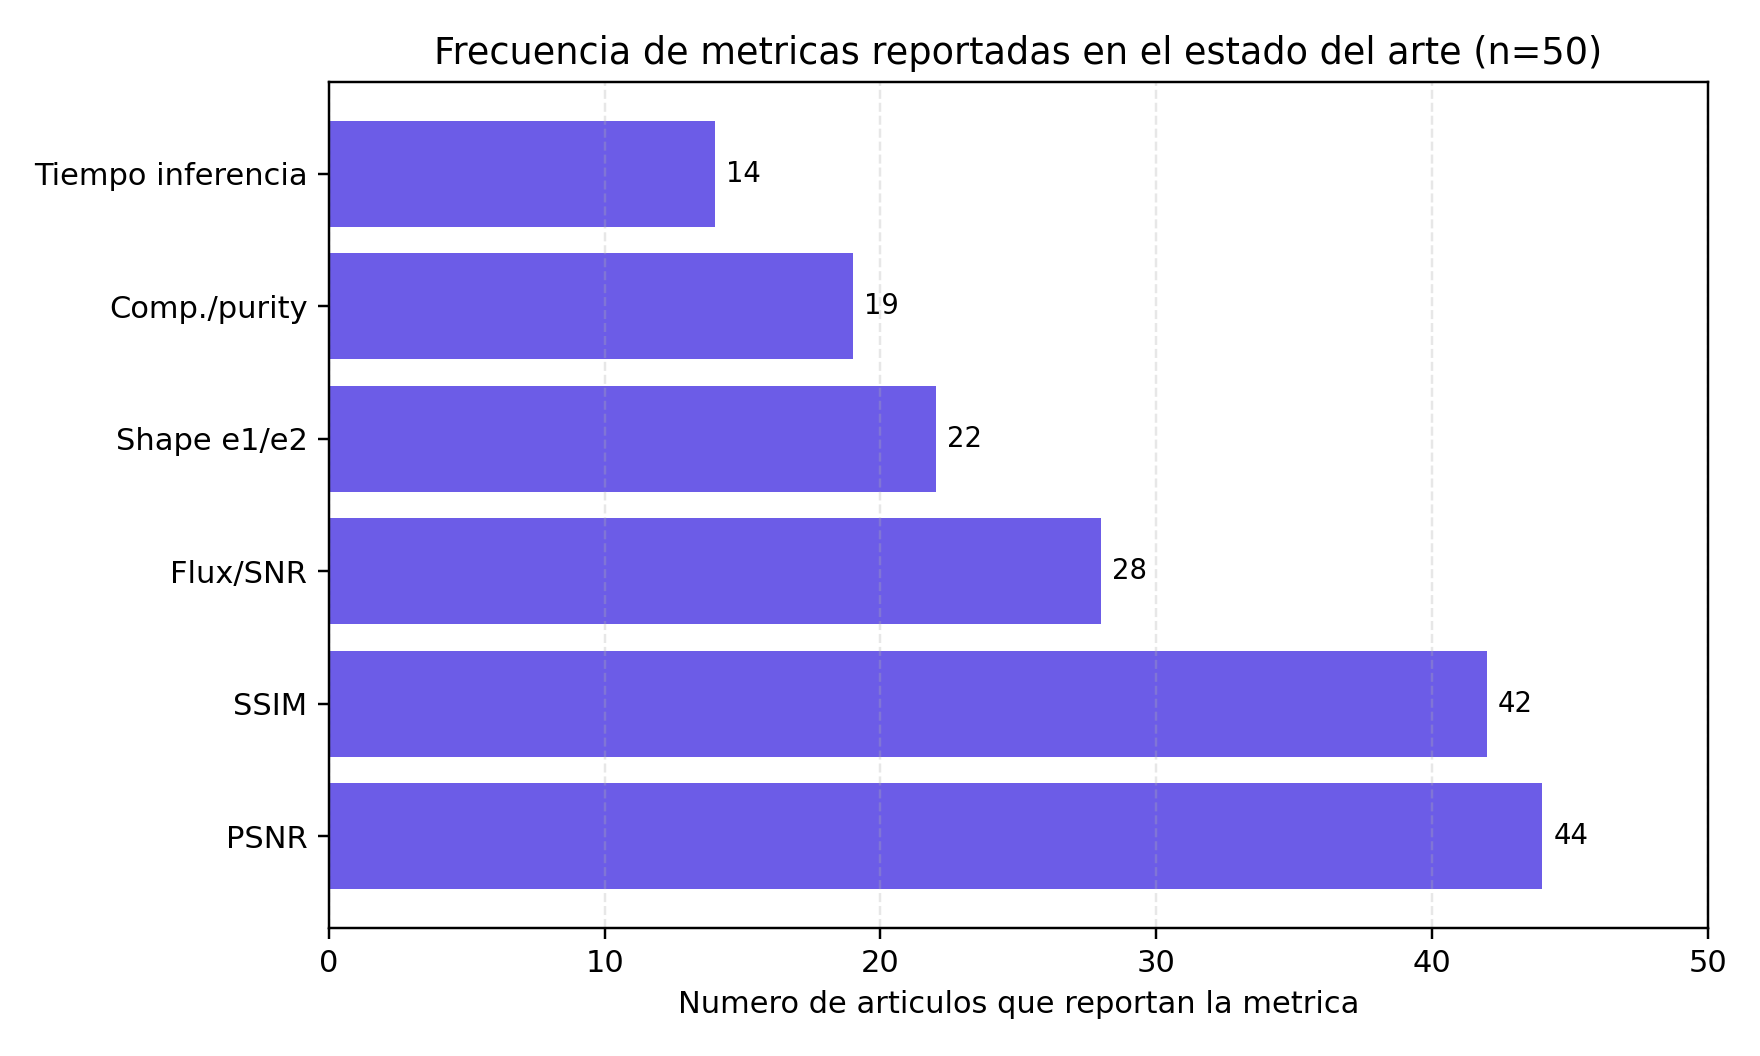
\includegraphics[width=0.9\linewidth]{assets/images/estado_arte_metricas_frecuencia.png}
    \caption{Frecuencia de m\'etricas reportadas en la literatura seleccionada (codificaci\'on cualitativa guiada por RAG + lectura manual).}
\end{figure}

\section{Clasificaci\'on t\'ecnica por enfoques}

\subsection{M\'etodos cl\'asicos y variacionales}
Los enfoques cl\'asicos siguen vigentes como referencia de interpretabilidad y estabilidad, especialmente en escenarios donde el modelo de ruido es conocido o parcialmente controlable \cite{roscani2020comparative, makarkin2021stateart, bui2023poisson}.

\subsection{CNN/U-Net supervisadas}
Las U-Net y variantes contin\'uan siendo un est\'andar de alto rendimiento para restauraci\'on de galaxias y deblending, con mejoras concretas en recuperaci\'on de se\~nal \'util para tareas de cat\'alogo \cite{vojtekova2020unet, hemmati2022deblending, park2024transformer, miao2024astrosr}.

\subsection{Auto-supervisi\'on y entrenamiento sin pares limpios}
Los m\'etodos auto-supervisados reducen la dependencia de datos ``clean'' perfectos, una limitaci\'on cr\'itica en astronom\'ia observacional \cite{liu2025selfsupervised, guo2026detection, sukurdeepa2025astroclearnet}.

\subsection{Modelos generativos y difusi\'on}
La familia de difusi\'on gana tracci\'on por su capacidad de modelar incertidumbre y mejorar escenarios de fondo complejo, incluyendo weak lensing y remoci\'on de ruido de fondo \cite{scognamiglio2025euclid, aoyama2025denoising, nicolaas2025bgrem, schanz2023diffusion, remy2023massmapping}.

\subsection{M\'etodos f\'isica-informados e h\'ibridos}
La integraci\'on de conocimiento instrumental (PSF, ruido CCD, fotometr\'ia multibanda) en arquitecturas profundas se consolida como tendencia de mayor valor para pipelines cient\'ificos robustos \cite{wang2022psf, sreejith2023psf, akhaury2022deep, akhaury2025joint, liu2026ccd}.

